% !TEX program = lualatex
\DocumentMetadata{pdfstandard=UA-2,pdfversion=2.0,lang=en-US,tagging=on}
\documentclass{./../../latex/tests}
\begin{document}
\thispagestyle{plain}
\myheader{Midterm 2 Sample: Solutions}
\rhead{Midterm 2 Sample: Solutions}
\vspace{0.5em}

\begin{enumerate}

%%%%%%%%%%%%%% Question 1
\item (5 pts)
\begin{enumerate}
\item (2 pts) The graph is the left half of the parabola $y = x^2$ joined at the origin to the ray $y = x$:

\begin{center}
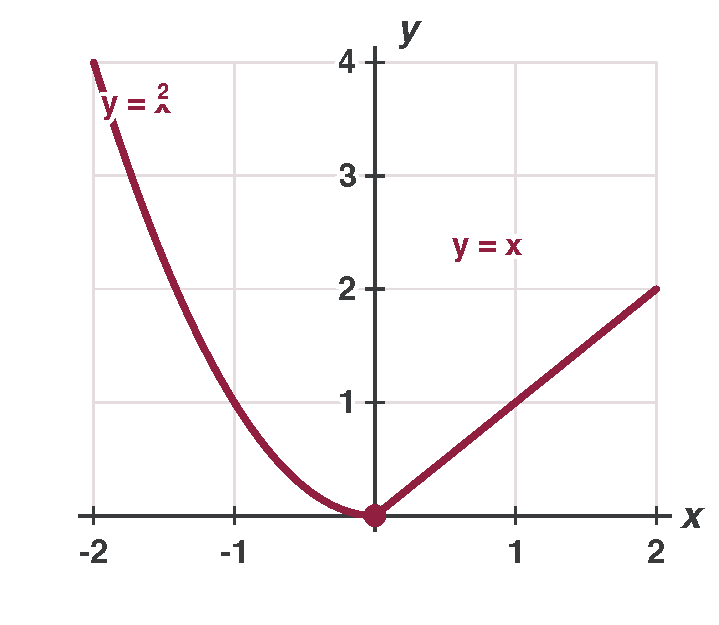
\includegraphics[width=0.42\textwidth,alt={Graph of the piecewise function: for x less than 0 the curve y equals x squared falls to the origin, and for x at least 0 the straight line y equals x rises from the origin, so the graph is connected but has a corner at the origin}]{../../latex/fig/kink.pdf}
\end{center}

\textbf{Continuous}: at $x = 0$ the left-side limit is $\lim_{x \rightarrow 0^-} x^2 = 0$, the right-side limit is $\lim_{x \rightarrow 0^+} x = 0$, and $f(0) = 0$, so the limit exists and equals $f(0)$. Away from $0$ each piece is a polynomial, so $f$ is continuous everywhere.

\textbf{Not differentiable} at $x = 0$: the slope from the left is $\lim_{x \rightarrow 0^-} 2x = 0$ while the slope from the right is $1$. The difference quotient has different left- and right-side limits, so $f'(0)$ does not exist: the graph has a corner at the origin.
\item (1 pt) By the chain rule (outer function $\ln u$, inner function $u = x^2 + 1$):
\[ f'(x) = \frac{1}{x^2 + 1} \cdot 2x = \frac{2x}{x^2 + 1} \]
\item (1 pt) By the quotient rule,
\[ f'(x) = \frac{5e^x(5x+e^x) - 5e^x(5+e^x)}{(5x+e^x)^2} = \frac{5e^x(5x - 5)}{(5x+e^x)^2} = \frac{25e^x(x-1)}{(5x+e^x)^2} \]
\item (1 pt) \[ \int_0^3 x^2 \, dx = \left[ \frac{x^3}{3} \right]_0^3 = \frac{27}{3} - 0 = 9 \]
\end{enumerate}

%%%%%%%%%%%%%% Question 2
\item (5 pts) $U(x, y) = x^{1/3} y^{2/3}$
\begin{enumerate}
\item (3 pts) \[ U_x = \frac{\partial U}{\partial x} = \frac{1}{3} x^{-2/3} y^{2/3} \qquad U_y = \frac{\partial U}{\partial y} = \frac{2}{3} x^{1/3} y^{-1/3} \]
\item (1 pt) Differentiate $U_x$ again:
\[ \frac{\partial U_x}{\partial x} = -\frac{2}{9} x^{-5/3} y^{2/3} < 0 \qquad \frac{\partial U_x}{\partial y} = \frac{2}{9} x^{-2/3} y^{-1/3} > 0 \]
So the marginal utility of $x$ is \textbf{decreasing} in $x$ (diminishing marginal utility) and \textbf{increasing} in $y$.
\item (1 pt) \[ dU = U_x\, dx + U_y\, dy = \frac{1}{3} x^{-2/3} y^{2/3}\, dx + \frac{2}{3} x^{1/3} y^{-1/3}\, dy \]
\end{enumerate}

%%%%%%%%%%%%%% Question 3
\item (5 pts) $\ln Q(p) = f(p)$
\begin{enumerate}
\item (2 pts) Differentiate both sides with respect to $p$:
\[ \frac{1}{Q(p)} \cdot \frac{dQ}{dp} = f'(p) \]
Multiply both sides by $p$:
\[ \varepsilon = \frac{dQ}{dp} \cdot \frac{p}{Q(p)} = p f'(p) \]
\item (2 pts) With $f(p) = 5 - 2 \ln p$, $f'(p) = -\dfrac{2}{p}$, so
\[ \varepsilon = p \cdot \left( -\frac{2}{p} \right) = -2 \]
Since $|\varepsilon| = 2 > 1$, demand is elastic, and at every price. (Equivalently, $Q = e^{5} p^{-2}$: a constant-elasticity demand curve.)
\item (1 pt) A 1\% increase in the price lowers the quantity demanded by about 2\%.
\end{enumerate}

%%%%%%%%%%%%%% Question 4
\item (5 pts)
\begin{enumerate}
\item (2 pts) $W$ depends on $t$ through both $A$ and $N$:
\[ \frac{dW}{dt} = \frac{\partial W}{\partial A} \frac{dA}{dt} + \frac{\partial W}{\partial N} \frac{dN}{dt} = 1 \cdot a + 1 \cdot ks e^{st} = a + ks e^{st} \]
\item (3 pts) Total cost is the integral of marginal cost:
\[ C(Q) = \int (2Q + 4)\, dQ = Q^2 + 4Q + c \]
The fixed cost pins down the constant: $C(0) = c = 10$, so
\[ C(Q) = Q^2 + 4Q + 10 \]
The increase in cost from $Q = 1$ to $Q = 3$ is
\[ \int_1^3 (2Q + 4)\, dQ = \left[ Q^2 + 4Q \right]_1^3 = (9 + 12) - (1 + 4) = 16 \]
Equivalently, $C(3) - C(1) = 31 - 15 = 16$.
\end{enumerate}

\end{enumerate}

\end{document}
